\documentclass[11pt]{article}

\usepackage[utf8]{inputenc}
\usepackage[T1]{fontenc}
\usepackage{lmodern}
\usepackage[margin=1in]{geometry}
\usepackage{graphicx}
\usepackage{booktabs}
\usepackage{amsmath}
\usepackage{microtype}
\usepackage[hidelinks]{hyperref}
\setlength{\emergencystretch}{3em}

\title{Living State Machine\\[4pt]
\large Gated, Ablatable Memory for Long-Horizon Preference Recall\\Around a Frozen Language Model}
\author{Kalen Patterson\\\small Independent research\\\small\texttt{kcpatterson27@gmail.com}}
\date{October 2026}

\begin{document}
\maketitle

\begin{abstract}
Long-horizon assistants need memory that is cheap, inspectable, and resistant to drift. This report describes \textbf{Living State Machine (LSM)}, a local-first wrapper around a frozen language model that combines a compact dual state, tiered episodic memory, habituation, Hebbian association, gated writes, a deterministic verifier, and surprise-modulated plasticity. Every mechanism is ablatable through configuration. On a matched-budget preference-recall benchmark, LSM scored \textbf{1.000} against \textbf{0.100} for naive retrieval-augmented generation across three seeds; a harder decoy-heavy stress benchmark was treated as a stress test rather than a success metric. The gated writer reached an F1 of \textbf{0.98} and was necessary under decoy load, where always-store collapsed to zero. The report also documents three substantive negative results---a multi-timescale memory variant, an encoder verifier, and a Stentor-style recurrent core---plus one evaluation-harness fault that initially looked like a model regression. The central claim is deliberately narrow: under a matched context budget, structured, gated memory can outperform naive retrieval. It is not a claim that the wrapper beats a full-context model on every long transcript.
\end{abstract}

\noindent\textbf{Keywords:} long-horizon memory; retrieval-augmented generation; gated writes; state-space models; local-first AI; evaluation hygiene

\section{Introduction}
A frozen language model is stateless between calls. The common workarounds are prompt stuffing, retrieval-augmented generation, or a separate memory service. Each buys context at a cost: full history grows without bound, retrieved snippets are brittle under decoys, and an LLM-written summary can quietly turn an assistant's guess into a persistent fact. On consumer hardware the constraint is sharper: a 12\,GB inference budget leaves little room for a second model to manage memory.

LSM studies a narrower question: can a compact set of inspectable, biologically inspired rules around a frozen model improve long-horizon preference recall at a \emph{matched context budget}? The system is a wrapper, not a fine-tune. It keeps a small working state $s_t$, a durable episodic store, and a per-turn control loop. The research track closed in July 2026; this report is a technical account of the evidence, including what failed.

The contributions are:
\begin{itemize}
  \item A wrapper architecture in which every memory mechanism has a \texttt{Null*} implementation, so ablations are configuration changes rather than rewrites.
  \item A deterministic facts-backed projection that replaces LLM-authored state after paraphrase errors were observed in live sessions.
  \item A gated writer and verifier layer, plus evidence that gating is what survives a decoy-heavy stress bench.
  \item A reproducible benchmark suite and a deliberately honest negative-results record, including a diagnosis of a false regression caused by one embedder choice.
\end{itemize}

\section{Related Work}
Retrieval-augmented generation (RAG) conditions a model on retrieved passages rather than the full corpus \cite{lewis2020rag}. It is effective when retrieval is clean, but it assumes the retrieved unit is useful in isolation. LSM instead retrieves from an episodic memory that has been filtered by a writer gate and scored by several signals.

Memory-augmented agents such as MemGPT treat the context window as a managed resource and move information between working and external memory \cite{packer2023memgpt}. Generative Agents maintain a memory stream with reflection and retrieval \cite{park2023generative}. LSM shares the tiered-memory premise but differs in two ways: the language model is frozen and local, and the persistent state is rendered deterministically from structured facts rather than authored by the model.

Long-context transformers reduce the need for retrieval by extending attention \cite{beltagy2020longformer}, while state-space models offer linear-time sequence mixing \cite{gu2023mamba}. LSM's Phase 2 explored a small state-space core, but the production path remained a wrapper; the trained core had to clear a no-regression gate rather than replace the baseline.

Habituation and associative learning are classic biological mechanisms \cite{thompson1966habituation}, and regularization methods for sequential learning address a related stability problem \cite{kirkpatrick2017ewc}. LSM borrows the vocabulary---habituation, association, surprise, plasticity---but evaluates each mechanism as an engineering component, not as a biological claim.

\section{System}

\subsection{Per-turn loop}
Each turn follows a fixed control loop: embed the turn; score memory candidates with cosine similarity, habituation damping, association boost, and trust; retrieve the top $k$; update the working state; compose a prompt from the state projection and retrieved snippets; call the frozen model; score the outcome; run the verifier; write only what passes the gate; and update plasticity signals. The loop is deliberately small enough to inspect in logs.

\begin{figure}[t]
\centering
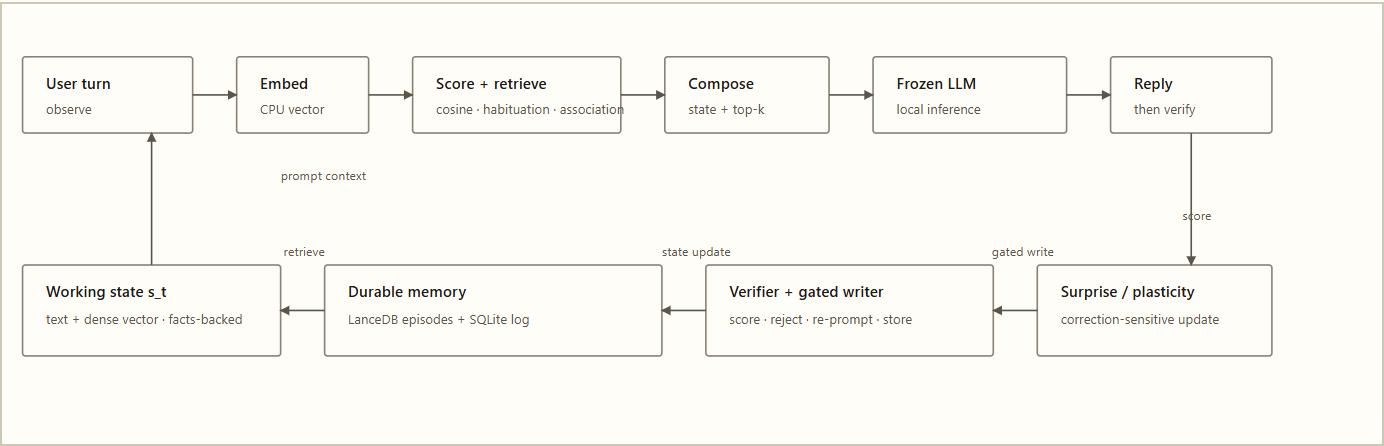
\includegraphics[width=\linewidth]{figure1.png}
\caption{The LSM control loop. The durable store is read through the scored retriever and written only through the verifier and gate. The working state is a compact projection, not a transcript.}
\label{fig:loop}
\end{figure}

\subsection{State and memory tiers}
$s_t$ is a dual representation: a short text projection injected into the prompt (roughly 400--600 characters) and a dense vector used for retrieval conditioning. Durable memory holds verbatim atoms in LanceDB plus an episodic SQLite log. Fast, session, and durable tiers are connected by promotion, hit-count, vitality decay, and a background consolidator. The mental model is explicit: the state is a compressed, inspectable summary; durable memory holds the evidence.

\subsection{Mechanisms}
Habituation damps repeated low-value input; association boosts memories that co-occur with the current turn; trust carries outcome history; surprise-modulated plasticity amplifies the learning rate on correction-like turns. The facts-backed updater renders \texttt{s\_t.text} deterministically from structured facts with recency, correction-aware slot ordering, and budget trimming. The LLM-authored summarizer remains only as an ablation. This change followed a live failure in which a vocative was absorbed into state as a game title and then inherited by every later turn.

\subsection{Gated writing and verification}
The verifier scores candidates rather than authoring text. Its five weighted components cover fact contradiction, identity drift, correction violation, list-merge errors, and length overflow. The score gates three surfaces: the writer (rejected text never becomes durable memory), the reply (one re-prompt with fix hints, then the lower-energy draft), and the legacy summarizer. The verifier is deterministic by default; a linear/hybrid learned head was evaluated, while an encoder variant was logged as a negative.

\subsection{Ablation as dependency injection}
Every mechanism sits behind a small Protocol with a \texttt{Null*} implementation. The eight benchmark configurations, the verifier family, and the state-updater family are therefore configuration flips. A run copies its YAML into the run directory with \texttt{metrics.json}, raw outputs, and logs; a run without its config is not treated as a run.

\section{Experimental Setup}
The evaluation suite contains eight tasks: matched-budget preference recall (\texttt{recall\_pref\_v1}), a harder decoy/long-gap stress task (\texttt{recall\_pref\_v2}), habituation and association signal benches, memory-write precision, multi-session consistency, fact correction, and verifier calibration. Headline claims use seeds 0, 1, and 2; Phase 2 integration checks are seed 0 only and are labelled as such.

The primary baselines are naive RAG and a raw LLM with a matched context budget. A full-transcript raw LLM is reported separately because it is not matched: it sees the entire history and therefore answers a different resource question. Hardware was a single RTX 5060 Ti (16\,GB VRAM, 32\,GB RAM) running a frozen local model through Ollama. A one-time cloud burst on a RunPod L40S cost approximately \textbf{\$8.04} and consumed about 9.3 hours for QLoRA and small-core training. The local test suite finished at 241 passed and 3 skipped.

\section{Results}

\begin{table}[t]
\centering
\small
\caption{Preference recall (accuracy; seeds 0--2). v2 is a stress bench, not the headline success metric.}
\label{tab:headline}
\begin{tabular}{lcc}
\toprule
System & \texttt{recall\_pref\_v1} & \texttt{recall\_pref\_v2} \\
\midrule
Naive RAG & 0.100 $\pm$ 0.100 & 0.044 $\pm$ 0.038 \\
Raw LLM, matched budget & 0.000 $\pm$ 0.000 & 0.000 $\pm$ 0.000 \\
Raw LLM, full transcript & 1.000 $\pm$ 0.000 & 0.911 $\pm$ 0.038 \\
\textbf{LSM full} & \textbf{1.000 $\pm$ 0.000} & 0.089 $\pm$ 0.038 \\
\bottomrule
\end{tabular}
\end{table}

On the matched-budget headline task, LSM reached the ceiling while naive RAG remained at 0.100. The full-context baseline also reached 1.000 on v1, so the result is not evidence that LSM beats full context on that task. On the harder v2 stress bench, the full-context model remained strong at 0.911 while LSM fell to 0.089; the matched raw baseline was 0.000. The honest reading is that v2 measures the value of full-history access, not a wrapper failure, and it is reported to keep the headline claim in bounds.

\begin{table}[t]
\centering
\small
\caption{Ablations on \texttt{recall\_pref\_v1} (seed 0--2 means). $\Delta$ is relative to LSM full.}
\label{tab:ablations}
\begin{tabular}{lccc}
\toprule
Ablation & Accuracy & $\Delta$ & Reading \\
\midrule
LSM full & 1.000 $\pm$ 0.000 & --- & Ceiling \\
No habituation & 0.967 $\pm$ 0.058 & $-$0.033 & Measured contribution \\
No writer gate & 0.933 $\pm$ 0.115 & $-$0.067 & Writer matters \\
Flat memory & 0.933 $\pm$ 0.058 & $-$0.067 & Tiering matters \\
No association & 1.000 $\pm$ 0.000 & 0.000 & Bench too easy \\
Multi-memory & 1.000 $\pm$ 0.000 & 0.000 & No separation \\
\bottomrule
\end{tabular}
\end{table}

\begin{table}[t]
\centering
\small
\caption{Component evidence: writer precision, retrieval MRR, and verifier calibration.}
\label{tab:components}
\begin{tabular}{lcl}
\toprule
Component & Result & Note \\
\midrule
Writer --- always & F1 0.67 & Precision 0.50, FPR 1.00 \\
Writer --- rules & F1 0.98 & Precision 1.00, recall 0.97, FPR 0.00 \\
Writer --- learned & F1 1.00 & 60 signal / 60 filler turns \\
Habituation signal & +0.068 MRR & 0.314 $\rightarrow$ 0.382 \\
Association signal & +0.317 MRR & 0.454 $\rightarrow$ 0.772 \\
Verifier --- rule & 0.556 macro-F1 & Default V.1 \\
Verifier --- linear/hybrid & 0.771 macro-F1 & $n=13$; directional only \\
Verifier --- encoder & 0.211 macro-F1 & Reject-all collapse; negative \\
\bottomrule
\end{tabular}
\end{table}

The Phase 2 integration gate held the headline benchmark at 1.000 when the trained hybrid SSM updater was projected into $s_t$, and both the Transformers base and the QLoRA adapter reached 1.000 after the harness fix described below. The trained core was therefore accepted as an optional state updater, not as a replacement for the wrapper.

\section{Negative Results and Failure Analysis}

\paragraph{Multi-timescale memory did not separate.}
A multi-timescale memory variant produced a small negative effect ($\Delta \approx -0.05$). The result was kept rather than tuned into the headline: on this bench, additional tiers added complexity without a measurable gain.

\paragraph{The encoder verifier collapsed.}
The MiniLM cross-encoder verifier scored 0.211 macro-F1 at $n=13$, effectively rejecting everything. With a small labeled set, the encoder had no room to learn the decision boundary. The linear and hybrid heads were retained as directional evidence; the encoder result is a named negative, not a hidden hyperparameter search.

\paragraph{Stentor-style recurrence lost to a minimal SSM.}
The ambitious Phase 2 hypothesis---that a Stentor-inspired recurrent core would beat a minimal diagonal SSM on language-modeling loss---failed: final loss was 5.21 versus 2.95 on TinyStories. The comparison was not clean: step counts and sequence lengths were unequal, and the association-trace update was sequential. The minimal core was promoted because it passed the no-regression gate, and the negative was logged with its confounds. The honest next experiment is a parallelized association scan at matched compute.

\paragraph{A false regression caused by the evaluation harness.}
After QLoRA training, the adapter path appeared broken: base 0.100 and +LoRA 0.200. The model was not the problem. A hash embedder combined with a minimum score of 0.15 filtered out the preference line, returning zero memories; switching the eval embedder to fastembed restored both paths to 1.000. The correction was written into the phase report. The lesson is now a first-class check: inspect retrieved-item counts before interpreting an end-to-end score.

\section{Limitations and Threats to Validity}
\begin{itemize}
  \item \textbf{Small, synthetic benchmarks.} The preference tasks are controlled and synthetic. They test a narrow memory behavior, not general assistant quality.
  \item \textbf{No external users.} Daily utility is a qualitative single-user observation; there is no retention or satisfaction study.
  \item \textbf{Seed asymmetry.} Headline results use three seeds; Phase 2 integration checks are seed 0 only. Treat those as directional.
  \item \textbf{Small verifier labels.} The learned/hybrid verifier result is $n=13$ and is not paper-grade. The encoder negative is similarly small.
  \item \textbf{Matched-budget scope.} The headline claim is about naive RAG at a matched budget. Full-context raw LLMs remain stronger on the harder stress bench.
  \item \textbf{Hardware and cost.} Results come from one consumer GPU and one approximately \$8 cloud burst; no multi-hardware replication.
  \item \textbf{Privacy boundary.} The system is local by default and supports optional encryption at rest, but the encryption path has not been independently audited.
  \item \textbf{Run artifacts.} The phase-report tables were reconciled with the repository on 2026-10-20. Raw run directories were not fully present in the review checkout, so the final artifact release should include them.
\end{itemize}

\section{Conclusion}
LSM shows that a compact, inspectable memory wrapper can produce a large gain over naive RAG at a matched context budget, and that the writer gate is the component most likely to matter when memory is under decoy pressure. The result is deliberately bounded: it does not claim to beat full-context models, and its negative results are part of the contribution. The next steps are matched-compute recurrence experiments, a larger verifier corpus, multi-seed Phase 2 integration, and a public, reproducible release of the code and run artifacts.

\section*{AI Assistance}
Text-to-text AI tools assisted with drafting, structuring, and editorial review. The author verified the measurements, tables, and citations and takes full responsibility for the content.

\section*{Code and Artifacts}
The implementation and run scripts are available from the author; a public artifact release is pending. The report's tables were reconciled against the Phase 1 and Phase 2 reports in the author's repository on 2026-10-20.

\begin{thebibliography}{9}
\bibitem{lewis2020rag}
P. Lewis et al., ``Retrieval-Augmented Generation for Knowledge-Intensive NLP Tasks,'' \emph{NeurIPS}, 2020. arXiv:2005.11401.

\bibitem{packer2023memgpt}
C. Packer et al., ``MemGPT: Towards LLMs as Operating Systems,'' 2023. arXiv:2310.08560.

\bibitem{park2023generative}
J. S. Park et al., ``Generative Agents: Interactive Simulacra of Human Behavior,'' \emph{UIST}, 2023. arXiv:2304.03442.

\bibitem{beltagy2020longformer}
I. Beltagy, M. E. Peters, and A. Cohan, ``Longformer: The Long-Document Transformer,'' 2020. arXiv:2004.05150.

\bibitem{gu2023mamba}
A. Gu and T. Dao, ``Mamba: Linear-Time Sequence Modeling with Selective State Spaces,'' 2023. arXiv:2312.00752.

\bibitem{thompson1966habituation}
R. F. Thompson and W. A. Spencer, ``Habituation: A Model Phenomenon for the Study of Neuronal Substrates of Behavior,'' \emph{Psychological Review}, 73(1):16--43, 1966.

\bibitem{kirkpatrick2017ewc}
J. Kirkpatrick et al., ``Overcoming Catastrophic Forgetting in Neural Networks,'' \emph{PNAS}, 114(13):3521--3526, 2017.
\end{thebibliography}

\end{document}
